\section{Intel 8086 Microprocessor}

This section consists of an implementation non-specific overview of the how the Intel 8086 is structured and functions at a high-level.

\subsection{General-Purpose and Index Registers}
    The Intel 8086 has four different 16-bit general-purpose registers (AX, BX, CX, DX), which can also be accessed as twice as many 8-bit registers (AL and AH, BL and BH, CL and CH, DL and DH). These registers can be used for any purpose but are implicitly used by many different instructions.

    There are also four 16-bit index registers on the 8086:
    \begin{itemize}
        \item Source Index (SI) - Points to the source in the current operation.
        \item Destination Index (DI) - Points to the destination in the current operation.
        \item Base Pointer (BP) - Points to the base of the stack within the stack segment.
        \item Stack Pointer (SP) - Points to the most recent value on the stack within the stack segment.
    \end{itemize}
    Note that unlike the general-purpose registers, the index registers are 16-bit only.

\subsection{Status Register/Flags}
    There are a set of flags in the 8086 that contain information about the state of the CPU. These flags are stored within a single 16-bit value, of which nine of those bits are used (see Table \ref{table:flags}).

    \begin{table}[h]
        \centering
        \begin{tabular} { | l c | c | m{0.6\textwidth} | }
            \hline
            Flags & & Bit & Purpose \\
            \hline
            Carry Flag              & (CF) &  0 & Set when an arithmetic operation resulted in a bit being carried. \\
            Parity Flag             & (PF) &  2 & Set if the binary representation of the result of the last operation is made up of an even number of bits. \\
            Axillary Carry Flag     & (AF) &  4 & Set when an arithmetic carry or borrow is generated out of the four least significant bits of an operation. \\
            Zero Flag               & (ZF) &  6 & Set when the result of the last arithmetic operation is equal to zero. \\
            Sign Flag               & (SF) &  7 & Set if the result of the last mathematical operation had its most significant bit set. \\
            Trap Flag               & (TF) &  8 & When set the processor will generate an internal interrupt after executing each instruction. This is for debugging purposes. \\
            Interrupt Flag          & (IF) &  9 & The processor will only recognise interrupt requests from peripherals when this flag is set. Otherwise, requests will be ignored. \\
            Direction Flag          & (DF) & 10 & Specifies the ordering of bytes when handling strings. \\
            Overflow Flag           & (OF) & 11 & Set when the last operation resulted in integer overflow. \\
            \hline
        \end{tabular}
        \caption{The nine different true/false flags stored in the FLAGS register.}
        \label{table:flags}
    \end{table}

\subsection{Memory Segmentation and Segment Registers}
    The 8086 has an unusual method of addressing up to one megabyte of memory. To find an absolute/physical address, the CPU shifts the 16-bit segment register four bits left and then adds the 16-bit offset address. Simply concatenating the segment and the offset to form a 32-bit absolute address, while slightly simpler, was deemed excessive for the time and would have required more expensive external bus pins.

    There are four different memory segments within the Intel 8086:
    \begin{itemize}
        \item Code Segment (CS) - The segment in which the executable program is stored. The instruction pointer is segmented within the code segment.
        \item Data Segment (DS) - Where any data used by the program is stored.
        \item Extra Segment (ES) - An additional area in which to store program data.
        \item Stack Segment (SS) - Where the contents of the stack is stored. All stack pointers (base pointer and stack pointer) are segmented within the stack segment.
    \end{itemize}

\subsection{Instruction Encoding}
    The x86 instruction set is an example of a Complex Instruction Set Computing (CISC) instruction set and it most certainly lives up to such a description. Each individual instruction can span from one to six bytes in length and is made up of several components which are outlined in the subsections below.

    \subsubsection{Opcode}
        While later x86 processors allowed for two byte opcodes, the 8086 only has 8-bit single byte opcodes. All instructions will have an opcode value and this value specifies what the instruction will do when executed as well as the ordering and types of parameters this instruction requires.

        The second-to-least significant bit of an opcode is known as the direction or \texttt{d} bit and is used to indicate whether the register specified within the instruction is a source (\texttt{d=0}) or a destination (\texttt{d=1}).

        The least significant bit of an opcode is known as the word or \texttt{w} bit and indicates whether the instruction will operate on 16-bit word values (\texttt{w=1}) or 8-bit byte values (\texttt{w=0}).

    \subsubsection{MOD-REG-R/M}
        Many instructions have a single MOD-REG-R/M byte immediately after the opcode. This byte specifies instruction operands and their addressing mode.

        \begin{figure}[h]
            \centering
            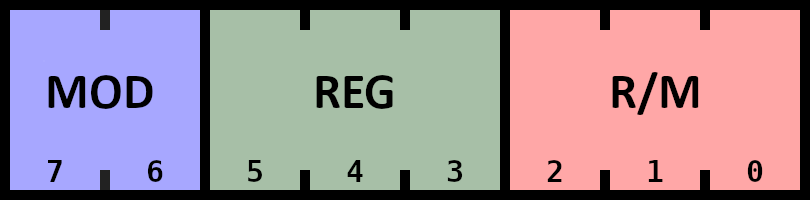
\includegraphics{mod-reg-rm}
            \caption{The structure of a MOD-REG-RM byte.}
            \label{figure:mod-reg-rm}
        \end{figure}

        As shown in Figure \ref{figure:mod-reg-rm} above, bits 7 and 6 of the MOD-REG-RM byte comprise the MOD component. These two bits specify the addressing mode used (see Table \ref{table:mod-addressing-mode}).

        \begin{table}[h]
            \centering
            \begin{tabular} { | c | m{0.7\textwidth} | }
                \hline
                MOD Value & Addressing Mode \\
                \hline
                00  & No displacement. \\
                01  & One byte displacement follows MOD-REG-R/M byte. \\
                10  & Two byte displacement follows MOD-REG-R/M byte. \\
                11  & R/M component is treated as a second register field (register addressing mode). \\
                \hline
            \end{tabular}
            \caption{Shows how the MOD bits of a MOD-REG-RM byte affect the addressing mode used.}
            \label{table:mod-addressing-mode}
        \end{table}

        Bits 3 to 5 make up the REG component of the MOD-REG-RM byte. This component specifies the register used (whether it is a source or destination is dependent on the `d` bit of the opcode). Table \ref{table:reg-addressing} shows which register will be used based on both the REG value and whether the instruction is operating on 8-bit or 16-bit values.

        \begin{table}[h]
            \centering
            \begin{tabular} { | c | m{0.1\textwidth} | m{0.1\textwidth} | }
                \hline
                REG Value & Register if 8-bit & Register if 16-bit \\
                \hline
                000 & AL & AX \\
                001 & CL & CX \\
                010 & DL & DX \\
                011 & BL & BX \\
                100 & AH & SP \\
                101 & CH & BP \\
                110 & DH & SI \\
                111 & BH & DI \\
                \hline
            \end{tabular}
            \caption{Show which register a REG value corresponds to (or R/M value when in register addressing mode as indicated by MOD value).}
            \label{table:reg-addressing}
        \end{table}

        The R/M part of the MOD-REG-RM byte is found in bits 0 to 2. When in register addressing mode (\texttt{MOD=11}), the R/M component, like the REG component, indicates a specific register (see table \ref{table:reg-addressing}). See the Displacement section below for the meaning of R/M when MOD is equal to other values.

    \subsubsection{Displacement}
        Depending on the value of MOD in the MOD-REG-RM byte, a instruction may be encode with up to two bytes of displacement. When MOD is either \texttt{01} or \texttt{10} (indicating either 8 or 16 bit displacement), the value of R/M will indicate against which index registers the displacement will be applied to (see table \ref{table:rm-values}).

        \begin{table}[h]
            \centering
            \begin{tabular} { | c | c | }
                \hline
                R/M Value & Operand Address \\
                \hline
                000 & BX + SI + Displacement \\
                001 & BX + DI + Displacement \\
                010 & BP + SI + Displacement \\
                011 & BP + DI + Displacement \\
                100 & SI + Displacement \\
                101 & DI + Displacement \\
                110 & BP + Displacement \\
                111 & BX + Displacement \\
                \hline
            \end{tabular}
            \caption{Shows the address used as an instruction operand based on R/M value (assuming MOD indicates that the R/M component is not being used as a second register field).}
            \label{table:rm-values}
        \end{table}

        Note that BX is the only general-purpose register which can also be used for indexing (as seen in table \ref{table:rm-values}).

    \subsubsection{Immediate}
        An immediate data value can be encoded directly into an instruction. This value can be a single byte or a 16-bit two byte value encoded in little endian (depending on the data size of the instruction).

\section{Intel 8259 Programmable Interrupt Controller (PIC)}
    The original Intel 8086 PCs relied upon a chip separate to the main Intel 8086 microprocessor called the Intel 8259. This chip managed several hardware interrupts (also known as Interrupt Requests or IRQs) and informed the processor when an interrupt required handling as well as which Interrupt Service Routine (ISR) should be called in order to do so. The Intel 8259 offered eight different interrupt pins numbered from 0 to 7 where IRQ 0 had highest priority while IRQ 7 the lowest.

    The 8259 PIC functions as something of a multiplexer as its eight possible interrupt pins fire just a single maskable interrupt pin on the processor. The processor will ignore all interrupt requests from the PIC indicated by the interrupt pin if its Interrupt Flag (IF) is set to 0. In this case, all external interrupts will effectively become disabled.

    \subsection{Registers}
        The 8259 PIC has three 8-bit registers which determine its behaviour.

        \subsubsection{Interrupt Mask Register (IMR)}
            The IMR allows for the individual interrupts provided by the PIC to be masked/disabled. The 8 bits of the IMR each correspond to an IRQ pin with the least significant bit corresponding to IRQ 0 and the most significant corresponding to IRQ 7. When an interrupt's masking bit within the IMR is set to 1, the interrupt will be masked meaning it will not be able to interrupt the processor. If an interrupt's bit is 0 however, then it will indeed interrupt the processor should the interrupt trigger.

        \subsubsection{Interrupt Request Register (IRR)}
            The IRR indicates when an interrupt has been fired. Like the IMR, each bit of the IRR corresponds to one of the eight interrupts. As soon as a device signals an interrupt then the appropriate bit in the IRR will be set to 1. This register can only be modified by the PIC itself.

        \subsubsection{In-Service Register (ISR)}
            The ISR indicates which interrupts are currently being serviced/handled (where execution has begun but is not complete).

    \subsection{Interrupt Vector Table}
        The Interrupt Vector Table holds the addresses for every interrupt handler that may be required by the system (both hardware and software interrupts). On the Intel 8086, this table always resides in memory from 0x0000 to 0x03FF and consists of 256 four-byte far pointers (two-byte segment and two-byte offset pairs).

    \subsection{Interrupt Firing/Handling}
        When an interrupt occurs, assuming the interrupt is not masked (in the IMR) and the processor has interrupts enabled (IF set), then the following takes place:
        
        \begin{itemize}
            \item The PIC asserts the processor's interrupt pin.
            \item Before it handles the interrupt, the processor finishes the execution of the current instruction.
            \item The processor sends a signal of acknowledgement back to the PIC who then in turn sends the vector number of the interrupt back to the processor.
            \item The vector number returned by the PIC is used as an index in the Interrupt Vector Table which is created by the BIOS. The corresponding entry in the interrupt vector table contains the address (segment and offset) for the appropriate interrupt service routine.
            \item The processor clears IF (disabling interrupts) and pushes FLAGS, CS and IP onto the stack.
            \item The processor then jumps to the address of the interrupt service routine by setting CS and IP to the segment address and offset respectively.
        \end{itemize}

\section{Intel 8253 Programmable Interval Timer (PIV)}
    The typical Intel 8086 system relies on a separate PIV chip in order for precise timing and counting functions. It offers three separate channels for this purpose labelled 0, 1 and 2.

    In IMB PC compatible devices, Timer Channel 0 fires INT 8 on IRQ 0 (highest priority interrupt offered). This channel is implemented as a descending counter where, once the initial value is set, it will repeatedly count down from that value. Computers running MS-DOS or similar operating systems typically have the first timer channel operate at a frequency of 18.2 Hz.

    \subsection{Control Word}
        The CPU is able to set the operating mode and format for each channel of the interval timer by writing an 8-bit control word to the PIT.

        The two most significant bits of the control word indicate (when not 11 as that is unused by the 8253) the channel this control word will affect (expressed in binary). The following two bits indicate the ordering of read and writes of the high/low bytes of the counter register. The next three bits indicate the timing mode (see table \ref{...}) while the final bit indicates whether the counter will operate in binary or binary-coded decimal (note that the latter is almost never used).

    \subsection{Modes}
        \subsubsection{Mode 0 (000)}
            In this mode, the counter will begin counting from the initial value in COUNT down to 0. Counting rate is equal to the input clock frequency. The OUT pin is set low after the control word is written, after which counting will begin a single cycle after COUNT is written to.

        \subsubsection{Mode 1 (001)}